
\scsection{Методологические проблемы современного состояния работ в области Искусственного интеллекта}
\label{intro_ostis}

\begin{SCn}

\scnsectionheader{\currentname}

\scnstartsubstruct

\scnsegmentheader{Начало раздела "\currentname"}

\scnstartsubstruct

\scnheader{Методологические проблемы современного состояния работ в области Искусственного интеллекта}

\scnrelfromvector{конкатенация сегментов}
{Структура деятельности в области Искусственного интеллекта;}
\scnauthorcomment{дополнить список}

\scnrelfromset{рассматриваемые вопросы}{
\scnfileitem{Каковы основные стратегические цели (сверхзадачи) научно-технической деятельности в области \textit{Искусственного интеллекта}?};
\scnfileitem{Какие проблемы являются на сегодняшний день актуальными для дальнейшего развития различных направлений \textit{Искусственного интеллекта} и для развития \textit{Искусственного интеллекта} в целом как общей (объединённой) \textit{научно-технической дисциплины}, а также для развития различных форм деятельности в этой области (научно-исследовательской деятельности создания технологий разработки интеллектуальных компьютерных систем, образовательной деятельности, бизнеса)?};
\scnfileitem{Какие проблемы являются на сегодняшний день актуальными для развития других \textit{научно-технических дисциплин} и являются ли эти проблемы аналогичными тем, которые актуальны для развития \textit{Искусственного интеллекта}?};
\scnfileitem{Какие можно предложить подходы к решению указанных выше проблем и как для этого можно использовать создаваемый сейчас новый технологический уклад в области \textit{Искусственного интеллекта} (следующий уровень технологий искусственного интеллекта)?};
\scnfileitem{Как будет выглядеть на основе следующего уровня \textit{технологий Искусственного интеллекта} комплексная автоматизация вех \textit{видов человеческой деятельности}, а также взаимодействие различных \textit{видов человеческой деятельности}, т.е. как будет выглядеть архитектура \textit{smart-общества}?};
\scnfileitem{Устраивает ли нас уровень семантической совместимости взаимопонимания между современными виртуальными компьютерными системами и что необходимо сделать для повышения этого уровня?};
\scnfileitem{Устраивает ли нас уровень семантической совместимости взаимопонимания между современными интеллектуальными компьютерными системами их пользователями и что необходимо сделать для повышения этого уровня?}}
\scntext{аннотация}{Предлагаемое вашему вниманию рассмотрение методологических проблем современного состояния работ в области \textit{Искусственного интеллекта} состоит из следующих частей:
\begin{scnitemize}
\item Анализ актуальных проблем, препятствующих дальнейшему развитию  \textit{Искусственного интеллекта} как \textit{научно-технической дисциплины}:
\begin{scnitemizeii}
\item Проблемы развития научных исследований в области \textit{Искусственного интеллекта} 
\item Проблемы разработки технологий проектирования и реализации \textit{интеллектуальных компьютерных систем};
\item Проблемы формирования рынка \textit{интеллектуальных компьютерных систем}; 
\item Образовательные проблемы в области \textit{Искусственного интеллекта};
\item Проблемы развития бизнеса в области \textit{Искусственного интеллекта}.
\end{scnitemizeii}
\item Анализ проблем автоматизации сложных видов деятельности:
\begin{scnitemizeii}
\item научно-исследовательской деятельности в рамках различных научных дисциплин;
\item создание \textit{технологий проектирования} и производства (реализации) сложных технических систем;
\item \textit{инженерной деятельности} по разработке сложных технических систем;
\item \textit{образовательной деятельности} по наукоёмким техническим специальностям
\end{scnitemizeii}
\item Формулировка принципов, лежащих в основе \textit{Технологии OSTIS}, предназначенной для решения указанных выше проблем;
\item Рассмотрение структуры \textit{Экосистемы OSTIS}, построенной по \textit{Технологии OSTIS} и обеспечивающей комплексную автоматизацию всех видов человеческой деятельности
\end{scnitemize}}

\scnrelfromset{используемые знаки общих понятий и иных сущностей}{деятельность\\
\scnaddlevel{1}
\scnidtf{область деятельности}
\scnsuperset{человеческая деятельность}
\scnaddlevel{-1}
;вид деятельности\\
\scnaddlevel{1}
\scnhaselement{проектирование}
\scnaddlevel{1}
\scnidtf{проектная деятельность}
\scnaddlevel{-1}
\scnhaselement{производство}
\scnaddlevel{1}
\scnidtf{производственная деятельность}
\scnaddlevel{-1}
\scnhaselement{наука}
\scnaddlevel{1}
\scnidtf{научная деятельность}
\scnaddlevel{-2}
;проект\\
\scnaddlevel{1}
\scnsuperset{открытый проект}
\scnaddlevel{-1}
;консорциум
;технология\\
\scnaddlevel{1}
\scnsuperset{информационная технология}
\scnaddlevel{1}
\scnsuperset{технология искусственного интеллекта}
\scnaddlevel{-2}
;кибернетическая система\\
\scnaddlevel{1}
\scnsuperset{интеллектуальная система}
\scnaddlevel{1}
\scnsuperset{интеллектуальная компьютерная система}
\scnaddlevel{1}
\scnidtf{искусственная интеллектуальная система}
\scnaddlevel{-3}
;конвергенция\scnsupergroupsign
\scnaddlevel{1}
\scnidtf{уровень конвергенции (близости)}
\scnsuperset{конвергенция кибернетических систем\scnsupergroupsign}
\scnaddlevel{-1}
;интеграция*\\
\scnaddlevel{1}
\scnsuperset{интеграция кибернетических систем*}
\scnsuperset{эклектичная интеграция*}
\scnsuperset{глубокая интеграция*}
\scnaddlevel{-1}
;интегрированная система\\
\scnaddlevel{1}
\scnsuperset{эклектичная система}
\scnsuperset{гибридная система}
\scnaddlevel{-1}
;экосистема интеллектуальных компьютерных систем
;рынок знаний\\
\scnaddlevel{1}
\scnidtf{рыночная организация порождения эволюции и применения знаний}
\scnaddlevel{-1}
;smart-общество\\
\scnaddlevel{1}
\scnidtf{общество,в основе которого лежит экосистема интеллектуальных компьютерных систем и рынок знаний}
\scnaddlevel{-1}
}
 
\scnrelfromset{ключевые знаки}
{Искусственный интеллект\\
\scnaddlevel{1}
\scniselement{научно-техническая дисциплина}
\scnaddlevel{1}
\scnsubset{научно-техническая деятельность} 
\scnaddlevel{-2};
интеллектуальная система\\
\scnaddlevel{1}
\scnsuperset{интеллектуальная компьютерная система}
\scnaddlevel{-1};
Общая теория интеллектуальных систем;
Базовая комплексная технология проектирования интеллектуальных компьютерных систем;
Технология производства спроектированных интеллектуальных компьютерных систем;
Специализированная инженерия в области Искусственного интеллекта;
Образовательная деятельность в области Искусственного интеллекта;
Бизнес-деятельность в области Искусственного интеллекта\bigskip;
\scnkeyword{Технология OSTIS};
\scnkeyword{ostis-система};
смысловое преставление информации;
агентно-ориентированная модель обработки информации в памяти; стандартизация ostis-систем;
\scnkeyword{SC-код};
абстрактная sc-машина;
конвергенция знаний в памяти;
ostis-систем;
конвергенция моделей решения задач в  ostis-системе;
интеграция знаний в памяти  ostis-системы;
интеграция моделей решения задач в  ostis-системе;
ostis-сообщество;
ostis-технология\\
\scnaddlevel{1}
\scnsuperset{ostis-технология проектирования}
\scnsuperset{ostis-технология производства}
\scnsuperset{технология эксплуатации ostis-систем}
\scnsuperset{технология реинжиниринга ostis-систем}
\scnaddlevel{-1};
\scnkeyword{Ядро Технологии OSTIS}\bigskip;
OSTIS-портал научных знаний в области Искусственного интеллекта;
Проект IMS.ostis;
\scnkeyword{Метасистема IMS.ostis};
Проект Программной реализации универсальной абстрактной sc-машины;
Проект разработки Универсального sc-компьютера;
Специализированная инженерия, осуществляемая на основе Технологии OSTIS;
Образовательная деятельность в области Искусственного интеллекта, осуществляемая на основе технологии OSTIS;
\scnkeyword{Консорциум OSTIS}\bigskip;
\scnkeyword{Экосистема OSTIS};
человеческая деятельность;
вид человеческой деятельности;
автоматизация человеческой деятельности;
качество человеческой деятельности;
субъект Экосистемы OSTIS;
Рынок знаний, реализованный в рамках Экосистемы OSTIS;
smart-общество}

\scnendstruct

    При необходимости, \textit{ostis-система} может включать не только компоненты, разработанные на основе \textit{Технологии OSTIS}, но и легко интегрироваться с любыми другими системами и интегрировать другие компоненты посредством специального протокола обмена информацией и/или программного интерфейса (API). Такие компоненты не будут в полной мере обладать некоторыми важными свойствами ostis-систем (например, рефлексивностью) но это позволит заимствовать современные разработки и решить проблему производительности при решении наиболее ресурсоемких задач (например, при обучении нейросетей).
    }
\scnaddlevel{-1}
\scnnote{Важно отметить, что \uline{\textit{OSTIS} -- не конкретная интеллектуальная система} или способ решения задач какого-либо класса, это \uline{технология разработки интеллектуальных систем}, каждая из которых в свою очередь в каждый конкретный момент будет решать задачи определенного класса. При этом ключевые преимущества \textit{OSTIS} заключаются не в принципиально новых функциональных возможностях разрабатываемых систем (большинство \textit{ostis-систем} могут быть реализованы современными традиционными средствами), а в том, насколько легко можно \uline{модифицировать и развивать} разрабатываемые системы, адаптировать их под новые задачи, а также в том, насколько эффективно можно \uline{накапливать и использовать полученные компоненты} при разработке новых систем, снижая при этом сроки и трудоемкость их разработки.
}
\filemodetrue
\scnrelfromvector{текущий состав}{программная реализация платформы (модели семантического компьютера), которая лежит в основе каждой ostis-системы. Может использоваться как при разработке web-приложений, так и настольных и мобильных приложений.;
постоянно пополняемая \textit{Библиотека компонентов баз знаний ostis-систем}, включая универсальное \textit{Ядро баз знаний ostis-систем}. В текущий момент наличие данной библиотеки позволяет сократить сроки разработки баз знаний на 40-60\%.;
постоянно пополняемая \textit{Библиотека компонентов решателей задач ostis-систем}, включая механизмы поиска информации и некоторые модели решения задач, среди которых выделяется соответствующее \textit{Ядро решателей задач ostis-систем}. В настоящее время на первых этапах разработки системы оказывается достаточным использовать только \textit{Ядро решателей задач ostis-систем} и не разрабатывать дополнительно никаких компонентов.;
комплекс \textit{Средств информационной поддержки разработчиков ostis-систем} (включая описание самих моделей, а также методики и руководства), оформленных в виде интеллектуальной \textit{Метасистемы IMS.ostis} (IMS) и доступный онлайн \url{https://ims.ostis.net.}}

\scnrelfromvector{текущее применение}{на основе \textit{Технологии OSTIS} силами студентов и аспирантов активно развивается большое число открытых прототипов обучающих и справочных систем, которые можно найти на \url{https://github.com/ostis-apps};
разработки на основе \textit{Технологии OSTIS} успешно внедрены на ОАО ``Савушкин продукт''  при разработке системы информационного обслуживания сотрудников и при разработке компонентов систем контроля качества продукции;
\textit{Технология OSTIS} позволит значительно более эффективно реализовать анализ естественного языка (включая речь), в том числе для чат-ботов, синхронного перевода и речевых ассистентов. В настоящее время выполняется ряд проектов по данной тематике.}
\filemodefalse
\scntext{планы развития}{Предполагается, что в ближайшем будущем \textit{Метасистема IMS.ostis} и другие \textit{ostis-системы} будут объединены в распределенную облачную \textit{ostis-систему}, названную \textit{Экосистемой OSTIS}. Общая архитектура экосистемы показана на рисунке \textit{Архитектура Экосистемы OSTIS}. При этом все \textit{ostis-системы} в составе \textit{Экосистемы OSTIS} будут в каждый момент времени совместимы между собой, при этом совместимость будет контролироваться автоматически. Любой желающий сможет внести свой вклад в развитие любой из ostis-систем в составе \textit{Экосистемы OSTIS}, в первую очередь -- \textit{Метасистемы IMS.ostis}, при этом вклад будет автоматически верифицироваться и оцениваться. В то же время, как видно из представленной архитектуры, владельцы \textit{ostis-систем} смогут самостоятельно выбирать, какой частью своей информации они готовы поделиться с другими пользователями \textit{Экосистемы OSTIS}, персональная же часть информации будет гарантированно защищена.}

\scnheader{Архитектура Экосистемы OSTIS}
\scneqimage{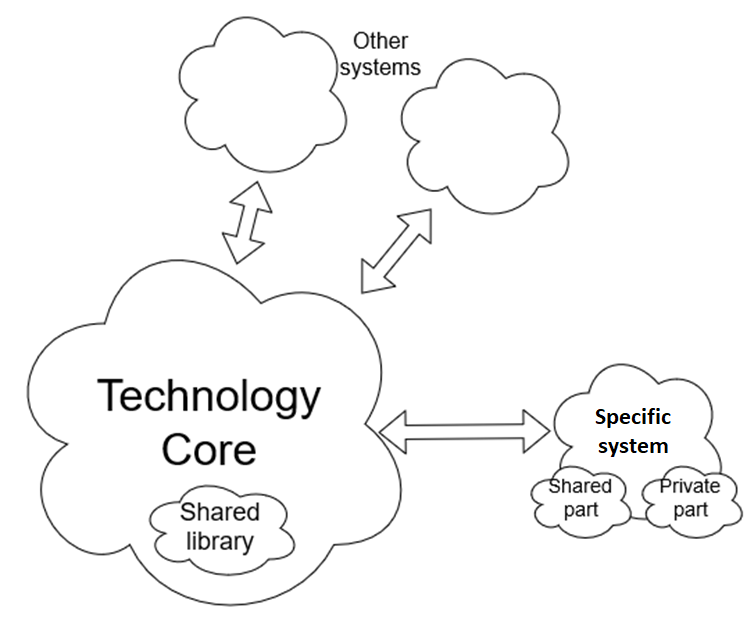
\includegraphics[width=0.6\textwidth]{figures/chapter0/ecosystem.png}}

\scnheader{Технология OSTIS}
\scnrelfromvector{текущие проекты}{Проект Экосистема OSTIS;Проект Метасистема IMS.ostis;Проект Семейство различных вариантов реализации универсального интерпретатора семантических моделей интеллектуальных систем\\
\scnaddlevel{1}
    \scnrelfromlist{подпроект}{Проект Программно реализованный на современных компьютерах универсальный интерпретатор семантических моделей интеллектуальных систем;Проект Семантический ассоциативный компьютер}
\scnaddlevel{-1}
;Проект Комплекс совместимых средств проектирования интеллектуальных систем\\
\scnaddlevel{1}
    \scnrelfromlist{подпроект}{Проект Встраиваемая типовая интеллектуальная система комплексной поддержки проектирования баз знаний;Проект Интеллектуальная система комплексной поддержки проектирования решателей задач интеллектуальных систем;Проект Интеллектуальная система комплексной поддержки проектирования вербальных интерфейсов интеллектуальных систем;Проект Интеллектуальная система комплексной поддержки проектирования невербальных интерфейсов}
\scnaddlevel{-1}
;Проект Семейство совместимых интеллектуальных справочных, обучающих и help-систем\\
\scnaddlevel{1}
    \scnrelfromlist{подпроект}{Проект Специализированные средства разработки совместимых интеллектуальных справочных, обучающих и help-систем различного назначения;Проект Комплекс семантически совместимых интеллектуальных справочных и обучающих систем по всем дисциплинам среднего образования;Проект Комплекс семантически совместимых интеллектуальных справочных и обучающих систем по всем дисциплинам, являющихся базовыми при подготовке инженеров по информационным специальностям;Проект Комплекс семантически совместимых интеллектуальных справочных и обучающих систем по всем специальным дисциплинам специальности ''Искусственный интеллект''{};Проект Семейство совместимых интеллектуальных справочных и обучающих систем по стандартам различного вида}
\scnaddlevel{-1}
;Проект Семейство совместимых интеллектуальных корпоративных систем ситуационного управления\\
\scnaddlevel{1}
    \scnrelfromlist{подпроект}{Проект Интеллектуальная корпоративная система ситуационного управления предприятием рецептурного производства;Проект Интеллектуальная корпоративная система ситуационного управления деятельностью выпускающей кафедры технического вуза}
\scnaddlevel{-1}
}
\scnrelfromvector{будущие проекты}{
Проект Семейство совместимых интеллектуальных систем автоматизации проектирования в различных областях;Проект Семейство совместимых порталов знаний\\
\scnaddlevel{1}
    \scnrelfrom{подпроект}{Проект Портал научных знаний по искусственному интеллекту}
\scnaddlevel{-1}
;Проект Семейство совместимых интеллектуальных систем экскурсионного обслуживания;Проект Семейство совместимых интеллектуальных геоинформационных систем;Проект Семейство совместимых интеллектуальных робототехнических систем и специализированных средств их разработки;Проект Семейство совместимых интеллектуальных систем персонального обслуживания и мониторинга\\
\scnaddlevel{1}
    \scnrelfromlist{подпроект}{Проект Интеллектуальная система персонального обслуживания и мониторинга пользователей и разработчиков компьютерных систем, входящих в Экосистему OSTIS;Проект Интеллектуальный персональный ассистент по взаимодействию с традиционными internet-системами и их пользователями;Проект Интеллектуальная система персонального комплексного медицинского мониторинга и контроля}
\scnaddlevel{-1}
}
\scnheader{конвергенция в области Искусственного интеллекта}

\scnrelfrom{разбиение}{Направления конвергенции в области Искусственного интеллекта}
     \scnaddlevel{1}
\scnhaselement{конвергенция Искусственного интеллекта со смежными научными дисциплинами}
    \scnaddlevel{1}
	\scnrelfrom{примечание}{\scnstartsetlocal\\
		\scnheaderlocal{Искусственный интеллект}
	\scnrelbothlist{смежная дисциплина}{Логика;Психология человека;Зоопсихология;Нейропсихология;Этология;Кибернетика;Общая теория систем;Семиотика;Лингвистика}
		\scnendstruct
	}
	\scnaddlevel{-1}

\scnhaselement{конвергенция различных направлений Искусственного интеллекта}
\scnaddlevel{1}
	\scnidtf{Конвергенция различных направлений исследований в области Искусственного интеллекта, результатом которой должна быть формализованная практически ориентированная общая теория интеллектуальных систем и, в частности, интеллектуальных компьютерных систем}
	\scnnote{Разобщенность различных направлений исследований в области искусственного интеллекта является главным препятствием создания общей комплексной технологии проектирования интеллектуальных компьютерных систем}
	\scnidtf{Конвергенция между различными направлениями и продуктами научных исследований в области искусственного интеллекта, результатом (целевым продуктом) которой должна стать общая формальная теория интеллектуальных компьютерных систем}
\scnaddlevel{-1}
\scnhaselement{конвергенция различного вида знаний в памяти интеллектуальной компьютерной системы}
\scnaddlevel{1}
	\scnidtf{Конвергенция и интеграция внутреннего представления в памяти интеллектуальной компьютерной системы различного вида знаний}
\scnaddlevel{-1}
\scnhaselement{конвергенция различных моделей решения задач в памяти интеллектуальной компьютерной системы}
\scnaddlevel{1}
	\scnidtf{Конвергенция и интеграция различных моделей решения задач, которая включает логико-семантическую типологию задач и типологию моделей решения задач и требует уточнения семантики таких понятий как задача, класс задач, метод, класс методов, модель решения задач (иерархический метод интерпретации класса методов)}
\scnaddlevel{-1}
\scnhaselement{конвергенция интеллектуальных компьютерных систем}
\scnaddlevel{1}
	\scnidtf{Обеспечение семантической совместимости (взаимопонимания) интеллектуальных систем, согласование используемых онтологий}
	\scnidtf{Конвергенция между различными прикладными компьютерными системами, результатом (целевым продуктом) которой должна стать экосистема, состоящая из перманентно эволюционирующих, семантически совместимых и взаимодействующих интеллектуальных компьютерных систем, а также их пользователей}
	\scnexplanation{Конвергенция (семантическая совместимость) всех разрабатываемых интеллектуальных компьютерных систем (в том числе прикладных), преобразующая набор индивидуальных (самостоятельных) интеллектуальных компьютерных систем различного назначения в коллектив активно взаимодействущих интеллектуальных компьютерных систем для совместного (коллективного) решения сложных (комплексных) задач и для перманентной поддержки семантической совместимости в ходе индивидуальной эволюции каждой интеллектуальной компьютерной системы.}
\scnaddlevel{-1}
\scnhaselement{конвергенция средств автоматизации проектирования различного вида компонентов интеллектуальных компьютерных систем}
\scnaddlevel{1}
	\scnidtf{Конвергенция (семантическая совместимость) средств автоматизации проектирования различного вида компонентов интеллектуальных компьютерных систем, результатом которой должен быть общий комплекс средств автоматизации проектирования всех компонентов интеллектуальных компьютерных систем}
	\scnidtf{Конвергенция между инструментальными средствами, обеспечивающими автоматизацию проектирования различных компонентов или различных классов интеллектуальных компьютерных систем, результатом (целевым продуктом) которой должен стать единый комплекс методологических и инструментальных средств, ориентированный на поддержку комплексного проектирования любых интеллектуальных компьютерных систем}
\scnaddlevel{-1}
\scnhaselement{конвергенция логико-семантических моделей интеллектуальных компьютерных систем}
\scnaddlevel{1}
	\scnnote{\textit{логико-семантические модели интеллектуальных компьютерных систем} являются результатом ("сухим"{} остатком) \textit{проектирования} этих систем и представляют собой формальное представления исходного (начального) состояния \textit{баз знаний} разрабатываемых \textit{интеллектуальных компьютерных систем}}
\scnaddlevel{-1}
\scnhaselement{конвергенция средств интерпретации логико-семантических моделей разрабатываемых интеллектуальных компьютерных систем}
\scnaddlevel{1}
\scnexplanation{Конвергенция (совместимость) средств реализации (производства) интеллектуальных компьютерных систем на основе спроектированных формальных моделей создаваемых интеллектуальных компьютерных систем (средств интерпретации спроектированных моделей интеллектуальных компьютерных систем). Такая интерпретация может осуществляться либо программным путем на современных компьютерах, либо путем создания принципиально новых компьютеров, специально ориентированных на интерпретацию формальных моделей интеллектуальных компьютерных систем, помещаемых в память указанных компьютеров}
\scnaddlevel{-1}
\scnhaselement{конвергенция между информационно-программным и 	аппаратным обеспечением интеллектуальных компьютерных систем}
\scnaddlevel{1}
	\scnidtf{Конвергенция между Software и Hardware интеллектуальных компьютерных систем}
\scnaddlevel{-1}
\scnhaselement{Конвергенция различных форм деятельности в области Искусственного интеллекта}
\scnaddlevel{1}
\scnexplanation{Конвергенция между
	\begin{scnitemize}
    \item научными исследованиями по созданию общей теории интеллектуальных компьютерных систем;
    \item разработкой средств автоматизации проектирования интеллектуальных компьютерных систем;
    \item разработкой средств интерпретации спроектированных формальных моделей интеллектуальных компьютерных систем;
    \item разработкой прикладных интеллектуальных компьютерных систем различного назначения;
    \item подготовкой и перманентным повышением квалификации кадров, способных эффективно участвовать во всех перечисленных направлениях деятельности.
    \end{scnitemize}
Глубокая конвергенция между всеми этими формами деятельности возможна только тогда, когда \uline{каждый} участник создания комплексной технологии искусственного интеллекта является участником \uline{каждой} из перечисленных форм деятельности.    
}
\scnidtf{Конвергенция между (1) научно-исследовательской деятельностью в области искусственного интеллекта; (2) инженерно-технологической деятельностью, которая направлена на разработку комплексной технологии проектирования интеллектуальных компьютерных систем и которая имеет высокий уровень наукоемкости; (3) инженерно-прикладной деятельностью, которая направлена на разработку прикладных интеллектуальных систем и которая также имеет высокий уровень наукоемкости, обусловленной необходимостью качественной формализации соответствующих предметных областей и, в частности, методов решения задач в этих областях; (4) образованием (образовательной деятельностью) в области искусственного интеллекта, повышение эффективности которого настоятельно требует раннего и поэтапного вовлечения студентов в реальные, а не учебные проекты - сначала в инженерно-прикладные, потом в инженерно- исследовательские проекты; (5) деятельностью, направленной на создание инфраструктуры, обеспечивающей поддержку открытого массового активного международного сотрудничества по консолидации усилий, направленных на решение современных проблем в области искусственного интеллекта; (6) бизнесом в области искусственного интеллекта, который не просто должен обеспечить финансовую поддержку перечисленных видов деятельности, но и обеспечить грамотный баланс между ними, грамотное сочетания тактических и стратегических целей}

\scnheader{Искусственный интеллект}
\scnrelfromset{методологические проблемы текущего состояния}{
\scnfileitem{Далеко не всеми учеными, работающими в области искусственного интеллекта принимается прагматичность практической направленности этой науки}
;\scnfileitem{Не всеми принимается необходимость конвергенции различных направлений искусственного интеллекта и необходимость их интеграции в целях построения общей теории интеллектуальных систем}
;\scnfileitem{Нет движения к построению общей компьютерной технологии интеллектуальных компьютерных систем}
;\scnfileitem{Нет движения к построению экосистем интеллектуальных компьютерных систем}
;\scnfileitem{Не всеми принимается необходимость конвергенции различных форм деятельности в области искусcтвенного интеллекта}}
\scnnote{Современная трактовка целей и задач Искусственного интеллекта как научно-технической дисциплины требует переосмысления, так как, к сожалению, носит несогласованный, а часто и значительно более узкий характер, чем этого требует текущее положение}


\scnheader{Бизнес-деятельность в области Искусственного интеллекта}
\scntext{текущее состояние}{Острая потребность в существенном повышении уровня автоматизации в самых различных областях человеческой деятельности (в промышленности, медицине, транспорте, образовании, строительстве и во многих других), а также современные результаты в развитии \textit{технологий Искусственного интеллекта} привели к существенному расширению работ по созданию \textit{прикладных интеллектуальных компьютерных систем} и к появлению большого количества коммерческих организаций, ориентированных на разработку таких приложений.}
\scnrelfromset{проблемы текущего состояния}{
\scnfileitem{Не так просто обеспечить баланс тактических и стратегических направлений развития всех форм деятельности в области \textit{Искусственного интеллекта} (научно-исследовательской деятельности, разработки технологии проектирования и производства интеллектуальных компьютерных систем, разработки прикладных систем, образовательной деятельности), а также баланс между всеми перечисленными формами деятельности.}
;\scnfileitem{В настоящее время отсутствует глубокая конвергенция различных форм деятельности в области \textit{Искусственного интеллекта} (в первую очередь, конвергенция развития технологий \textit{Искусственного интеллекта} и разработки различных прикладных интеллектуальных компьютерных систем), что существенно затрудняет развитие каждой из этих форм.}
;\scnfileitem{Высокий уровень наукоемкости работ в области \textit{Искусственного интеллекта} предъявляет особые требования к квалификации сотрудников и к их способности работать в составе творческих коллективов.}
;\scnfileitem{Для повышения квалификации своих сотрудников и для обеспечения высокого уровня своих разработок необходимо активное сотрудничество с различными научными школами, с кафедрами, осуществляющими подготовку молодых специалистов в области \textbf{\textit{Искусственного интеллекта}}, активное участие в подготовке и проведении соответствующих конференций, семинаров, выставок.}}

\scnheader{Искусственный интеллект}
\scnrelfromset{сверхзадачи текущего состояния}{
\scnfileitem{Построение и перманентное развитие \textit{общей формальной теории интеллектуальных систем}}
\scnaddlevel{1}
\scnrelfromset{подзадачи}{
\scnfileitem{Уточнение требований, предъявляемых к интеллектуальным компьютерным системам – уточнение свойств интеллектуальных компьютерных систем, определяющих высокий уровень их интеллекта.}
;\scnfileitem{Конвергенция и интеграция всевозможных видов знаний и всевозможных моделей решения задач в рамках каждой интеллектуальной компьютерной системы.}
;\scnfileitem{Ориентация на последующую разработку унифицированных семантически совместимых формальных моделей интеллектуальных систем.}
;\scnfileitem{Ориентация на разработку различного вида универсальных интерпретаторов формальных моделей интеллектуальных систем (и в том числе компьютеров нового поколения ) и обеспечение четкой стратификации между формальными моделями интеллектуальных систем и различными вариантами построения их интерпретаторов, обеспечивающей высокую степень независимости эволюции формальных моделей интеллектуальных систем и эволюции их интерпретаторов. Это требует особой детализации формальных моделей интеллектуальных систем.}
;\scnfileitem{Обеспечение коммуникационной ("социальной"{}) совместимости (договороспособности) интеллектуальных компьютерных систем, позволяющей им самостоятельно формировать коллективы интеллектуальных компьютерных систем и их пользователей, а также самостоятельно согласовывать (координировать) деятельность в рамках этих коллективов при решении сложных задач в непредсказуемых условиях. Без этого невозможна реализация таких проектов, как "умный"{} дом, "умный"{} город, "умное"{} предприятие, "умная"{} больница и т.д.}}
\scnaddlevel{-1}
;\scnfileitem{Создание и перманентное развитие \textit{общей комплексной технологии} проектирования и производства \textit{семантически совместимых} \scnbigspace \textit{интеллектуальных компьютерных систем}, способных координировать свою деятельность с себе подобными}
\scnaddlevel{1}
\scnrelfromset{подзадачи}{
\scnfileitem{Четкое описание стандарта интеллектуальных компьютерных систем, обеспечивающего семантическую совместимость разрабатываемых систем}
;\scnfileitem{Разработка мощных библиотек семантически совместимых и многократно (повторно) используемых компонентов разрабатываемых интеллектуальных компьютерных систем}
;\scnfileitem{Обеспечение низкого порога вхождения в технологию проектирования интеллектуальных компьютерных систем как для пользователей технологии (т.е. разработчиков прикладных или специализированных интеллектуальных компьютерных систем), так и для разработчиков самой технологии}
;\scnfileitem{Обеспечение высоких темпов развития технологии за счет учета опыта разработки различных приложений путем активного привлечения авторов приложений к участию в развитии (совершенствовании) технологии}}
\scnaddlevel{-1}
;\scnfileitem{Разработка компьютеров нового поколения, ориентированных на производство высокопроизводительных \textit{интеллектуальных компьютерных систем} самого различного назначения и высокого качества}
;\scnfileitem{Создание глобальной \textit{экосистемы} взаимодействующих между собой \textit{интеллектуальных компьютерных систем}, обеспечивающих комплексную автоматизацию всех \textit{видов человеческой деятельности}}
\scnaddlevel{1}
\scntext{подзадача}{Построение формальной модели человеческой деятельности в контексте теории smart-общества}
\scnaddlevel{-1}
;\scnfileitem{Создание и перманентное развитие глобальной \textit{социотехнической экосистемы}, которая состоит из \textit{интеллектуальных компьютерных систем}, а также всех пользователей этих систем, которая обеспечивает комплексную автоматизацию всех \textit{видов человеческой деятельности}}
;\scnfileitem{Необходим переход от эклектичного построения сложных \textit{интеллектуальных компьютерных систем}, использующих различные виды \textit{знаний} и различные виды \textit{моделей решения задач}, к их глубокой \textbf{интеграции} и унификации, когда одинаковые модели представления и модели обработки знаний реализуется в разных системах и подсистемах одинаково}
;\scnfileitem{Необходимо сократить дистанцию между современным уровнем \textbf{\textit{теории интеллектуальных компьютерных систем}} и практики их разработки.}}

\scnheader{Искусственный интеллект}
\scnidtf{Деятельность в области Искусственного интеллекта (как совокупность всех форм и направлений этой деятельности)}
\scntext{проблема текущего состояния}{Эпицентром современных проблем развития деятельности в области \textit{Искусственного интеллекта} является \textit{конвергенция} и \textit{глубокая интеграция} всех форм, направлений и результатов этой деятельности. Уровень взаимосвязи, взаимодействия и \textit{конвергенции} между различными формами и направлениями деятельности в области \textit{Искусственного интеллекта} явно недостаточен. Это приводит к тому, что каждая из них развивается обособленно, независимо от других.  Речь идет о \textit{конвергенции} между такими направлениями \textit{Искусственного интеллекта}, как представление знаний, решение интеллектуальных задач, интеллектуальное поведение, понимание и др., а также между такими формами \textit{человеческой деятельности в области Искусственного интеллекта}, как научные исследования, разработка технологий, разработка приложений, образование, бизнес. 
Почему на фоне уже достаточно длительного интенсивного развития научных исследований в области \textit{Искусственного интеллекта} до сих пор не создан рынок интеллектуальных компьютерных систем и комплексная технология \textit{Искусственного интеллекта}, обеспечивающая разработку широкого спектра \textit{интеллектуальных компьютерных систем} самого различного назначения и доступной широкому контингенту инженеров. 
Потому что сочетание высокого уровня наукоемкости и прагматизма этой проблемы требует для ее решения принципиально нового подхода к организации взаимодействия \textit{\uline{ученых}}, работающих в области \textit{Искусственного интеллекта}, \textit{\uline{разработчиков}} средств автоматизации проектирования \textit{интеллектуальных компьютерных систем}, \uline{\textit{разработчиков}} средств реализации интеллектуальных компьютерных систем, включая средства аппаратной поддержки интеллектуальных компьютерных систем, \uline{\textit{разработчиков}} прикладных интеллектуальных компьютерных систем. Такое \uline{целенаправленное} взаимодействие должно осуществляться как в рамках каждой из этих форм деятельности в области \textit{Искусственного интеллекта}, так и между ними. Таким образом, основной тенденцией дальнейшего развития теоретических и практических работ в области \textit{Искусственного интеллекта} является конвергенция как самых разных видов (форм и направлений) человеческой деятельности в области \textit{Искусственного интеллекта}, так и самых разных продуктов (результатов) этой деятельности. Необходимо ликвидировать барьеры между различными видами и продуктами деятельности в области \textit{Искусственного интеллекта} в целях обеспечения их совместимости и интегрируемости.
Проблема создания быстро развивающегося рынка семантически совместимых интеллектуальных систем – это вызов, адресованный специалистам в области \textit{Искусственного интеллекта}, требующий преодоления "вавилонского столпотворения"{} во всех его проявлениях, формирование высокой культуры договороспособности и унифицированной, согласованной формы представления коллективно накапливаемых, совершенствуемых и используемых знаний.
Ученые, работающие в области \textit{Искусственного интеллекта}, должны обеспечить конвергенцию результатов различных направлений \textit{Искусственного интеллекта} и построить: (1) общую теорию интеллектуальных компьютерных систем; (2) общую технологию проектирования семантически совместимых интеллектуальных компьютерных систем, включающую соответствующие стандарты интеллектуальных компьютерных систем и их компонентов. Инженеры, разрабатывающие интеллектуальные компьютерные системы, должны сотрудничать с учеными и участвовать в развитии технологии проектирования интеллектуальных компьютерных систем.}

\newpage
\scnsegmentheader{Понятие Технологии OSTIS}

\scnstartsubstruct

\scnheader{Технология OSTIS}
\scnidtf{Комплекс (семейство) технологий, обеспечивающих проектирование, производство, эксплуатацию и реинжиниринг интеллектуальных \textit{компьютерных систем} (\textit{ostis-систем}), предназначенных для автоматизации самых различных видов человеческой деятельности и в основе которых лежит смысловое представление и онтологическая систематизация знаний, а также агентно-ориентированная обработка знаний}
\scnidtf{Open Semantic Technology for Intelligent Systems}
\scnaddlevel{1}
\scntext{сокращение}{OSTIS}
\scnaddlevel{-1}
\scnidtf{Семейство (комплекс) \textit{ostis-технологий}}
\scnidtf{Комплексная открытая семантическая технология проектирования, производства, эксплуатации и реинжиниринга гибридных, семантически совместимых, активных и договороспособных \textit{интеллектуальных компьютерных систем}}
\scnrelfromset{принципы, лежащие в основе}{
\scnfileitem{Ориентация на разработку \textit{интеллектуальных компьютерных систем}, имеющих высокий уровень \textit{интеллекта} и, в частности, высокий уровень \textit{социализации}. Указанные системы, разработанные по \textit{Технологии OSTIS}, будем называть \textbf{\textit{ostis-системами}}}
;\scnfileitem{Ориентация на \uline{комплексную} автоматизацию всех видов и областей \textit{человеческой деятельности} путем создания сети взаимодействующих и координирующих свою деятельность \textit{ostis-систем}. Указанную сеть \textit{ostis-систем} вместе с их пользователями будем называть \textbf{\textit{Экосистемой OSTIS}}}
;\scnfileitem{Поддержка перманентной эволюции \textit{ostis-систем} в ходе их эксплуатации.}
;\scnfileitem{\textit{Технология OSTIS} реализуется в виде сети \textit{ostis-систем}, которая является частью \textit{Экосистемы OSTIS}.
Ключевой \textit{ostis-системой} указанной сети является \textbf{\textit{Метасистема IMS.ostis}} (Intelligent MetaSystem), реализующая \textbf{\textit{Ядро Технологии OSTIS}}, которое включает в себя базовые (предметно независимые) методы и средства проектирования и производства \textit{ostis-систем} с интеграцией в их состав типовых встроенных подсистем поддержки эксплуатации и реинжиниринга \textit{ostis-систем}. Остальные \textit{ostis-системы}, входящие в состав рассматриваемой сети, реализуют различные специализированные \textit{ostis-технологии} проектирования различных классов \textit{ostis-систем}, обеспечивающих автоматизацию любых областей и \textit{видов человеческой деятельности}, кроме \textit{проектирования ostis-систем}.}
;\scnfileitem{Конвергенция и интеграция на основе смыслового представления знаний всевозможных научных направлений \textit{Искусственного интеллекта} (в частности, всевозможных базовых знаний и навыков решения интеллектуальных задач) в рамках \textit{Общей формальной семантической теории ostis-систем}.}
;\scnfileitem{Ориентация на разработку компьютеров нового поколения, обеспечивающих эффективную (в том числе производительную) интерпретацию логико-семантических моделей \textit{ostis-систем}, которые представлены базами знаний этих систем, имеющими смысловое представление.}}

\scnendstruct

\bigskip
\scnfragmentcaption

\scnheader{Понятие ostis-системы}

\scnstartsubstruct

\scnheader{ostis-система}
\scnidtf{\textit{интеллектуальная компьютерная система}, спроектированная и реализованная по требованиям и стандартам \textit{Технологии OSTIS}, которые задокументированы в \textit{Общей теории ostis-систем}}
\scnidtf{Множество \textit{ostis-систем} различного назначения}
\scnaddlevel{1}
\scniselement{имя собственное}
\scnaddlevel{-1}
\scnidtf{Множество всевозможных \textit{интеллектуальных компьютерных систем}, построенных по \textit{Технологии OSTIS}}
\scnsubset{интеллектуальная компьютерная система}
\scnidtf{\textit{интеллектуальная компьютерная система}, которая построена в соответствии с требованиями и стандартами \textit{Технологии OSTIS}, что обеспечивает существенное развитие целого ряда \textit{свойств} (способностей) этой \textit{компьютерной системы}, позволяющих значительно повысить \textit{уровень интеллекта} этой системы (и, прежде всего, ее \textit{уровень обучаемости} и \textit{уровень социализации})} 

\scnauthorcomment{Добавить классификацию из пояснения к Технологии OSTIS}

\scnsubdividing{индивидуальная ostis-система;коллективная ostis-система\\
\scnaddlevel{1}
    \scnsubdividing{простой коллектив ostis-систем;иерархический коллектив ostis-систем}   
\scnaddlevel{-1}
}

\scnnote{Когда речь идет о таком компоненте Технологии OSTIS, как Общая теория ostis-систем, имеется в виду строгое формальное уточнение того, как устроена \textit{ostis-система}, какова ее архитектура, принципы организации памяти, принципы организации представления и обработки информации, принципы организации интерфейса с внешней средой (в том числе, с пользователями)}

\scnrelfromset{принципы, лежащие в основе}{
\scnfileitem{Хранение информации в памяти \textit{ostis-системы} ориентируется на \uline{смысловое} представление информации -- без синонимии и омонимии знаков, без семантической эквивалентности информационных конструкций.}
;\scnfileitem{Абстрактная память \textit{ostis-системы} является графодинамической (т.е. нелинейной (графовой) и структурно перестраиваемой). Переработка информации в памяти \textit{ostis-системы} сводится не столько к изменению состояния элементов памяти (это происходит только при изменении синтаксического типа элементов и при изменении содержимого тех элементов, которые обозначают файлы), сколько к изменению \uline{конфигурации связей} между ними.}
;\scnfileitem{Ориентация на компьютеры нового поколения.}
;\scnfileitem{В основе организации решения задач в памяти \textit{ostis-системы} лежит \textit{агентно-ориентированная модель обработки информации}, управляемая ситуациями и событиями, возникающими в обрабатываемой информации (точнее, в обрабатываемой \textit{базе знаний}). С точки зрения архитектуры \textit{ostis-система} представляет собой \uline{иерархическую} многоагентную систему с общедоступной памятью (т.е. с памятью, общедоступной \uline{всем} агентам \textit{ostis-системы}).\\
Заметим при этом, что общая память большинства исследуемых в настоящее время \textit{многоагентных систем} является не общедоступной, а распределенной, т.е. представляет собой абстрактное (виртуальное) объединение, в состав которого входит память каждого агента многоагентной системы. Координация деятельности агентов \textit{ostis-системы} при выполнении сложных \textit{действий в памяти} \scnbigspace \textit{ostis-системы} реализуется также через \textit{память ostis-системы} с помощью хранимых в памяти \textit{методов} решения различных \textit{классов задач}, а также с помощью хранимых в памяти \textit{планов} решения конкретных задач.\\
На основании этого можно строить неограниченную иерархическую систему \textit{агентов ostis-системы} -- от элементарных агентов, обеспечивающих выполнение базовых действий в памяти \textit{ostis-системы}, до неэлементарных агентов, представляющих собой коллективы (группы) элементарных и/или неэлементарных агентов, обеспечивающих решение различных типовых задач с помощью соответствующих методов и планов.}
;\scnfileitem{Реализация децентрализованного ситуационного управления деятельностью ostis-систем не только на уровне внутренних информационных процессов, но также на уровне организации индивидуальной деятельности во внешней среде и даже на уровне участия в коллективной деятельности в рамках различных коллективов ostis-систем. Организация выполнения \textit{ostis-системой действий во внешней среде} осуществляется следующим образом:
\begin{scnitemize}
	\item Выделяются классы \textit{элементарных действий во внешней среде}, для реализации каждого из которых вводятся \textit{эффекторные агенты} ostis-системы.
	\item Координация деятельности \textit{эффекторных агентов} ostis-системы при выполнении \textit{сложных действий во внешней среде} осуществляется через \textit{память ostis-системы} с помощью хранимых в памяти \textit{методов} и \textit{планов} решения различных задач во \textit{внешней среде}, а также с помощью \textit{рецепторных агентов} ostis-системы, обеспечивающих обратную связь и, соответственно, сенсомоторную координацию.
\end{scnitemize}}
;\scnfileitem{Унификация базового набора (базовой системы) используемых \textit{понятий}, что является основой обеспечения \textit{семантической совместимости} всех \textit{ostis-систем}.}
;\scnfileitem{В основе структуризации информации (\textit{базы знаний}), хранимой в памяти \textit{ostis-системы}, лежит иерархическая система \textit{предметных областей} и соответствующих им \textit{формальных онтологий}.}
;\scnfileitem{Способность к пониманию (к семантическому погружению, к семантической интеграции) новых приобретаемых знаний (и, в том числе, новых навыков) в состав текущего состояния \textit{базы знаний}.}
;\scnfileitem{Способность к \textit{семантической конвергенции} (к обнаружению сходств) новых приобретаемых знаний (и, в частности, навыков) со знаниями, входящими в состав текущего состояния \textit{базы знаний} \textit{ostis-системы}.}
;\scnfileitem{Способность к интеграции различных видов знаний.}
;\scnfileitem{Способность к интеграции различных моделей решателей задач.}
;\scnfileitem{Способность ostis-систем понимать друг друга, а также любого своего пользователя путем согласования системы используемых понятий (по терминам и по денотационной семантике). Способность \textit{ostis-системы} обеспечивать и поддерживать высокий уровень своей \textit{семантической совместимости} (высокий уровень взаимопонимания) с другими \textit{ostis-системами} в процессе собственной эволюции, а также эволюции других ostis-систем, которая приводит к расширению и/или корректировке системы используемых понятий.}
;\scnfileitem{Способность ostis-системы согласовывать, координировать свою деятельность с другими системами при решении задач, которые усилиями одной (индивидуальной) интеллектуальной компьютерной системы не могут быть решены либо принципиально, либо за разумное время.}
;\scnfileitem{Высокая степень индивидуальной обучаемости ostis-систем, обеспечиваемая высокой степенью их гибкости, стратифицированности, рефлексивности, а также универсальностью средств представления и образования знаний.}
;\scnfileitem{Высокая степень коллективной обучаемости ostis-систем, обеспечиваемая высокой степенью их семантической совместимости.}
;\scnfileitem{\scnauthorcomment{статья на OSTIS-2020}}}
\scnaddlevel{1}
\scntext{следовательно}{Перечисленные свойства \textit{ostis-систем} свидетельствуют о том, что они имеют существенно более высокий \textit{уровень интеллекта} и, в частности, более высокий \textit{уровень социализации} по сравнению с современными \textit{интеллектуальными компьютерными системами}. \scnauthorcomment{См. начало Раздела 1.1}}
\scnaddlevel{-1}

\bigskip
\scnmakeset{память*;ostis-система}
\scnrelfrom{сужение второго домена заданного отношения для заданного первого домена}{память ostis-системы}
\scnaddlevel{1}
\scnsubset{смысловая память}
\scnaddlevel{-1}

\bigskip
\scnmakeset{информация, хранимая в памяти кибернетической системы*;  ostis-система}
\scnrelfrom{сужение второго домена заданного отношения для заданного первого домена}{база знаний ostis-системы}
\scnaddlevel{1}
\scnsubset{смысловое представление информации}
\scnaddlevel{-1}

\scnheader{решатель задач ostis-системы }
\scnsubset{агентно-ориентированная модель обработки информации в памяти}

\newpage
\scnsegmentheader{Текущее состояние и проблемы дальнейшего развития деятельности в области Искусственного интеллекта}
\scnstartsubstruct

\scntext{аннотация}{Рассмотрим в каких направлениях должна происходить эволюция повышенного качества деятельности в области \textit{Искусственного интеллекта}, а также эволюция продуктов этой деятельности}

\bigskip
\scnfragmentcaption

\scnheader{Научно-исследовательская деятельность в области Искусственного интеллекта}
\scntext{текущее состояние}{}
\scnauthorcomment{добавить из статей}

\scnheader{Научно-исследовательская деятельность в области Искусственного интеллекта}
\scnrelfromset{проблемы текущего состояния}{
\scnfileitem{Отсутствует согласованность систем \textit{понятий} в разных направлениях \textit{Искусственного интеллекта} и, как следствие, отсутствует \textit{семантическая совместимость} и \textit{конвергенция} этих направлений, в результате чего ни о каком движении в направлении построения \textit{общей теории интеллектуальных систем} с высоким уровнем формализации и речи быть не может. Существование и продолжающееся увеличение "высоты барьеров"{} между различными направлениями исследований в области \textit{Искусственного интеллекта} проявляется в том, что специалист, работающий в рамках какого-либо направления \textit{Искусственного интеллекта}, посещая заседания "не своей"{} секции на конференции по \textit{Искусственному интеллекту}, мало что там может понять и, соответственно, извлечь полезного для себя.};
\scnfileitem{Отсутствует мотивация и осознание острой необходимости в указанной \textit{конвергенции} между различными направлениями \textit{Искусственного интеллекта}.};
\scnfileitem{Отсутствует реальное движение в направлении построения \textit{Общей теории интеллектуальных систем}, поскольку отсутствует соответствующая мотивация и осознание острой практической необходимости в этом.}
}

\bigskip
\scnfragmentcaption

\scnheader{Разработка базовой комплексной технологии проектирования интеллектуальных компьютерных систем}
\scntext{текущее состояние}{Современная технология \textit{Искусственного интеллекта} представляет собой целое семейство всевозможных частных технологий, ориентированных на разработку и сопровождение различного вида компонентов \textit{интеллектуальных компьютерных систем}, реализующих самые различные модели представления и обработки информации, различные модели решения задач, ориентированных на разработку различных классов \textit{интеллектуальных компьютерных систем}.}
\scnrelfromset{проблемы текущего состояния}{
\scnfileitem{высокая трудоемкость разработки интеллектуальных компьютерных систем};
\scnfileitem{необходимая высокая квалификация разработчиков};
\scnfileitem{современные технологии \textit{Искусственного интеллекта} принципиально не обеспечивают разработки таких \textit{интеллектуальных компьютерных систем}, в которых устраняются недостатки современных \textit{интеллектуальных компьютерных систем}};
\scnfileitem{совместимость частных технологий \textit{Искусственного интеллекта} практически отсутствует и, как следствие, отсутствует \textit{семантическая совместимость} разрабатываемых \textit{интеллектуальных компьютерных систем}, поэтому их системная интеграция осуществляется \uline{вручную}.};
\scnfileitem{Разрабатываемые \textit{интеллектуальные компьютерные системы} не способны \uline{самостоятельно} координировать свою деятельность друг с другом следовательно
\begin{scnitemize}
\item{нет общей комплексной технологии проектирования интеллектуальных компьютерных систем};
\item{не обеспечивается совместимость и взаимодействие разрабатываемых систем (синтаксическая и семантическая совместимость)};
\item{нет совместимости между существующими частными технологиями проектирования различных компонентов интеллектуальных компьютерных систем (базы знаний, нейросетевые модели, интеллектуальные интерфейсы и т.д.)};
\item{есть инструментальные средства по компонентам, но "склеивать"{} (соединять, интегрировать) это надо вручную};
\item{нет системы инструментальных средств}
\end{scnitemize}
}
}

\bigskip
\scnfragmentcaption

\scnheader{Разработка технологии производства спроектированных интеллектуальных компьютерных систем}
\scntext{текущее состояние}{Был сделан целый ряд попыток разработки \textit{компьютеров} нового поколения, ориентированных на использование в \textit{интеллектуальных компьютерных системах}. Но все они оказались неудачными, так как не были ориентированы на всё многообразие моделей решения задач в \textit{интеллектуальных компьютерных системах}. В этом смысле они не были \textit{\uline{универсальными} компьютерами} для \textit{интеллектуальных компьютерных систем}.}
\scnrelfromset{проблемы текущего состояния}{
\scnfileitem{Разрабатываемые \textit{интеллектуальные компьютерные системы} могут использовать самые различные комбинации \textit{моделей решения интеллектуальных задач} (логических моделей, соответствующих различного вида логикам, нейросетевых моделей различного вида, моделей целеполагания, синтеза планов, моделей управления сложными объектами, моделей понимания и синтеза текстов естественного языка и т.д.). Современные (традиционные, фон-неймановские) \textit{компьютеры} не в состоянии достаточно производительно интерпретировать всё многообразие указанных моделей решения задач. При этом разработка специализированных \textit{компьютеров}, ориентированных на интерпретацию какой-либо одной модели решения задач (нейросетевой модели или какой-либо логической модели) проблему не решает, так как в \textit{интеллектуальной компьютерной системе} необходимо использовать сразу несколько разных моделей решения задач, причём в различных сочетаниях.}
}

\bigskip
\scnfragmentcaption

\scnheader{Специализированная инженерия в области Искусственного интеллекта}
\scnidtf{Деятельность, направленная на разработку \textit{интеллектуальных компьютерных систем} различного назначения с использованием имеющихся для этого моделей, методов и средств}
\scnidtf{Деятельность по проектированию и производству \textit{интеллектуальных компьютерных систем}}
\scnidtf{Деятельность, направленная на формирование рынка \textit{интеллектуальных компьютерных систем}}
\scnrelfrom{в перспективе}{Специализированная инженерия в области \textit{Искусственного интеллекта}, осуществляемая специальной частью Экосистемы OSTIS}
	\scnaddlevel{1}
	\scnrelfrom{продукт}{Экосистема OSTIS}
	\scnrelfrom{субъект действия}{часть Экосистемы OSTIS, осуществляющая специализированную инженерию в области \textit{Искусственного интеллекта}}
	\scnaddlevel{-1}

\scntext{текущее состояние}{}
\scnauthorcomment{добавить из статей}

\scnrelfromset{проблемы текущего состояния}{
\scnfileitem{Отсутствует четкая систематизация многообразия \textit{интеллектуальных компьютерных систем}, соответствующая систематизации автоматизируемых \textit{видов человеческой деятельности}.};
\scnfileitem{Отсутствует \textit{конвергенция} \scnbigspace \textit{интеллектуальных компьютерных систем}, обеспечивающих автоматизацию \textit{областей человеческой деятельности}, принадлежащих одному и тому же \textit{виду человеческой деятельности}.};
\scnfileitem{Отсутствует \textit{семантическая совместимость}(семантическая унификация, взаимопонимание) между \textit{интеллектуальными компьютерными системами}, основной причиной чего является отсутствие согласованной системы общих используемых \textit{понятий}.};
\scnfileitem{Семантическая недружественность \textit{пользовательского интерфейса} и отсутствие встроенной справочной системы, позволяющей запрашивать информацию об элементах интерфейса и возможностях системы, приводят к низкой эффективности эксплуатации всех возможностей \textit{интеллектуальной компьютерной системы}.};
\scnfileitem{Анализ проблем автоматизации всех \textit{видов человеческой деятельности} убеждает в том, что дальнейшая автоматизация \textit{человеческой деятельности} требует не только повышения уровня \textit{интеллекта} соответствующих \textit{интеллектуальных компьютерных систем}, но и реализации их способности
\begin{scnitemize}
\item устанавливать свою \textit{семантическую совместимость} (взаимопонимание) как с другими \textit{компьютерными системами}, так и со своими пользователями\char59
\item поддерживать эту \textit{семантическую совместимость} в процессе собственной эволюции, а также эволюции пользователей и других \textit{компьютерных систем}\char59
\item координировать свою деятельность с пользователями и другими \textit{компьютерными системами} при коллективно решении различных задач\char59
\item участвовать в распределении работ (подзадач) при коллективном решении различных задач.
\end{scnitemize}
Важно подчеркнуть то, что реализация вышеперечисленных способностей создаст возможность для существенной и даже полной автоматизации \textit{системной интеграции} \scnbigspace \textit{компьютерных систем} в комплексы взаимодействующих систем и автоматизации реинжиниринга таких комплексов. Такая автоматизация системной интеграции и её реинжиниринга:
\begin{scnitemize}
\item даст возможность комплексам кибернетических систем \uline{самостоятельно} адаптироваться к решению новых задач\char59
\item существенно повысит эффективность эксплуатации таких комплексов компьютерных систем, так как реинжиниринг системной интеграции компьютерных систем, входящих в такой комплекс, часто востребован (например, при реконструкции предприятия)\char59
\item существенно сокращает число ошибок по сравнению с "ручным"{} (неавтоматизированным) выполнением \textit{системной интеграции} и её \textit{реинжиниринга}, которые, к тому же, требует высокой квалификации.
\end{scnitemize}
Таким образом следующий этап повышения уровня автоматизации \textit{человеческой деятельности} настоятельно требует создания таких \textit{интеллектуальных компьютерных систем}, которые могли бы легко сами (без системного интегратора) объединяться для совместного решения сложных задач. 
}
}

\bigskip
\scnfragmentcaption

\scnheader{Образовательная деятельность в области искусственного интеллекта}
\scntext{текущее состояние}{Целенаправленная подготовка специалистов в области Искусственного интеллекта имеет богатую историю и осуществляется во многих ведущих университетах (Stanford University, MIT, МГУ (Москва), НИУ МЭИ (Москва), РГГУ (Москва), СПбГУ (Санкт-Петербург), ДВФУ (Владивосток), НГТУ (Новосибирск), НТУУ КПИ (Киев), БГУИР (Минск), БГУ (Минск), БрГТУ (Брест) и других).}
\scnrelfromset{проблемы текущего состояния}{
\scnfileitem{Поскольку деятельность в области \textit{Искусственного интеллекта} сочетает в себе и высокую степень наукоемкости и высокую степень сложности инженерных работ, подготовка специалистов в этой области требует одновременного формирования у них как научно-исследовательских навыков, культуры и стиля мышления, так и инженерно-практических навыков, культуры и стиля мышления. С точки зрения методики и психологии обучения сочетание фундаментальной научной и инженерно-практической подготовки специалистов является весьма сложный образовательной педагогической задачей.};
\scnfileitem{Отсутствует \textit{семантическая совместимость} между различными учебными дисциплинами, что приводит к "мозаичности"{} восприятия информации};
\scnfileitem{Отсутствует системный подход к подготовке молодых специалистов в области \textit{Искусственного интеллекта}};
\scnfileitem{Нет персонификации обучения};
\scnfileitem{Нет установки на выявление, раскрытие и развитие таланта творческого проектирования};
\scnfileitem{Отсутствует целенаправленное формирование мотивации к творчеству};
\scnfileitem{Нет формирования навыков работы в реальных коллективах разработчиков};
\scnfileitem{Отсутствует адаптация к реальной практической деятельности};
\scnfileitem{Любая современная технология (в том числе и Технология OSTIS) должна иметь высокие темпы своего развития, поскольку без этого невозможно поддерживать высокий уровень её конкурентоспособности. Но для быстро развиваемой технологии требуется:
\begin{scnitemize}
\item не просто высокая квалификация кадров, использующих и развивающих технологию,
\item но и высокие \uline{темпы} повышения уровня этой квалификации, так как без этого невозможно эффективно использовать и развивать \uline{быстро меняющуюся} технологию.
\end{scnitemize}
\bigskip
Из этого следует, что образовательная деятельность в области \textit{Искусственного интеллекта} и соответствующая ей технология должна быть не просто важной частью деятельности в области \textit{Искусственного интеллекта}, а частью, глубоко интегрированной во все остальные виды деятельности в области \textit{Искусственного интеллекта}. Так, например, каждая \textit{интеллектуальная компьютерная система} должная быть ориентирована не только на обслуживание своих конечных пользователей, не только на организацию целенаправленного взаимодействия со своими разработчиками, которые постоянно совершенствуют эту систему, и не только на обеспечение минимального "порога вхождения"{} для новых конечных пользователей и разработчиков, но и на организацию постоянного и персонифицированного повышения квалификации каждого своего конечного пользователя и разработчика в условиях постоянных изменений, вносимых в указанную \textit{интеллектуальную компьютерную систему}. Для этого эксплуатируемая \textit{интеллектуальная компьютерная система} должна "знать"{}, что в ней изменилось, на что она способна и как эти способности инициировать (содержание и форма, соответствующих пользовательских команд)
}
}

\scnendstruct

\newpage
\scnheader{смысловое представление информации}
\scnrelfromset{принципы, лежащие в основе}{
\scnfileitem{Каждый синтаксически элементарный (атомарный) фрагмент представленной информации является обозначением некоторой сущности, которая может быть реальной или абстрактной, конкретной (фиксированной, константной) или произвольной (переменной), постоянной или временной, четкой (достоверной) или нечеткой (недостоверной с возможным дополнительным уточнением степени правдоподобности).}
	\scnaddlevel{1}
\scntext{следовательно}{В состав смыслового представления информации не могут входить буквы, слова, словосочетания, разделители, ограничители}
	\scnaddlevel{-1}
;\scnfileitem{В рамках смыслового представления информации отсутствует синонимия (пары синонимичных знаков), омонимия  (омонимичные знаки), семантическая эквивалентность (пары семантически эквивалентных информационных конструкций), т.е. отсутствует любая форма дублирования информации, а также отсутствует неоднозначность соотношения между знаками и их денотатами.}}
	\scnaddlevel{1}
\scntext{следовательно}{Смысловое представление информации не может выглядеть как цепочка (строка, последовательность) синтаксически элементарных фрагментов, поскольку каждая описываемая сущность и взаимно однозначно соответствующий ей ее знак может быть связана не с двумя, а с любым количеством описываемых сущностей. Другими словами, смысловое представление информации является нелинейной (графовой) информационной конструкцией.}
		\scnaddlevel{1}
\scntext{следовательно}{Если внутреннее представление информации в памяти компьютерной системы является смысловым представлением, то обработка информации в такой памяти носит графодинамический характер и сводится не к изменению состояния элементов памяти, а к изменению конфигурации связей между ними.}
	\scnaddlevel{-2}
\scnnote{Ключевая проблема современного этапа развития общей теории интеллектуальных компьютерных систем и технологии их разработки – это проблема обеспечения \textbf{\textit{семантической совместимости}} 
\begin{enumerate}
	\item различных видов знаний, входящих в состав баз знаний интеллектуальных компьютерных систем;
	\item различных видов моделей решателей задач;
	\item различных интеллектуальных компьютерных систем в целом;
\end{enumerate}
Для решения этой проблемы очевидно необходима унификация (стандартизация) формы представления знаний в памяти интеллектуальных компьютерных систем. Предлагаемым нами подходом для такой унификации и является ориентация на \textbf{смысловое представление информации (знаний)} в памяти интеллектуальных компьютерных систем. Основой предполагаемого нами подхода к обеспечению высокого уровня обучаемости т семантической совместимости интеллектуальных компьютерных систем, а также к разработке стандарта интеллектуальных компьютерных систем является унификация \textbf{смыслового представления информации (знаний)} в памяти интеллектуальных компьютерных систем и построение глобального \textbf{смыслового пространства} знаний.}
\scnaddlevel{1}
\scnnote{Информация в знаковой конструкции в основном содержится не в самих знаках (в их структуре), а в связях между знаками. При этом существенно, чтобы эти связи (синтаксические связи) имели четкую смысловую (семантическую) интерпретацию. 
Если структура знаков содержит информацию об обозначаемой сущности всегда можно заменить на «бесструктурные» знаки, которые имеют семантическую окружность} 

\scnheader{семантическая сеть}
\scnsubset{смысловое представление информации}
\scnexplanation{Семантическая сеть нами рассматривается не как красивая метафора сложноструктурированных знаковых конструкций, а как формальное уточнение понятия смыслового представления информации, как принцип представления информации, лежащей в основе нового поколения компьютерных языков и самих компьютерных систем – графовых языков и графовых компьютеров.}

\scnheader{семантическая сеть}
\scnsubset{знаковая конструкция}
\scnexplanation{Семантическая сеть – это знаковая конструкция, обладающая следующими свойствами:
	\begin{scnitemize}
		\item «внутренняя» структура (строение) знаков, входящих в семантическую сеть; не требуется учитывать при ее семантическом анализе (понимании)
		\item Смысл семантической сети определяется денотационной семантикой всех входящих в нее знаков и конфигурацией связей инцидентности этих знаков
		\item Из двух инцидентных знаков, входящих в семантическую сеть, один является знаком связи
		\item Синонимия, омонимия
	\end{scnitemize}
}

\scnheader{семантическая сеть}
\scnrelfrom{предлагаемый подход}{\textbf{SC-код}}
	\scnaddlevel{1}
	\scnidtf{Предлагаемое в рамках \textit{Технологии OSTIS} уточнение понятия \textit{семантической сети}}
	\scnaddlevel{-1}
\scnsuperset{SC-код}
	\scnaddlevel{1}
	\scnidtf{Semantic Computer Code}
	 \scnrelfromlist{смотрите}{Раздел 0.3.2; Раздел 2.1.1.1}
	 
\scnheader{многоагентная система}
\scnsubset{кибернетическая система}
\scnexplanation{Кибернетическая система, представляющая собой множество кибернетических систем, способных коммуницировать, т.е. обмениваться информацией друг с другом (причем не обязательно каждый с каждым)}

\scnheader{агент*}
\scnidtf{агент многоагентной системы*}

\scnheader{внешняя среда*}
\scnidtf{внешняя среда кибернетической системы}

\scnheader{память*}
\scnidtf{внутренняя (информационная) среда кибернетической системы}
\scnnote{Не каждая кибернетическая система (в том числе многоагентная система) имеет явно выделенную память, являющуюся хранилищем накапливаемой информации, накапливаемого опыта.}

\scnheader{многоагентная система}
\scnsubdividing{многоагентная система без общей памяти;многоагентная система с общей памятью}
\scnsubdividing{многоагентная система, в которой управление агентами осуществляется только путем обмена сообщениями между ними;многоагентная система, в которой управление агентами осуществляется через общую для них память}
\scnsubdividing{многоагентная система с централизованным управлением агентами;многоагентная система с децентрализованным управлением агентами}
\scnsubdividing{многоагентная система, в которой областью деятельности всех ее агентов является только внешняя среда этой системы;многоагентная система, в которой областью деятельности ее агентов является как внешняя среда, так и память этой системы\\
	\scnaddlevel{1}	
\scnnote{некоторые агенты такой системы могут работать только в памяти}}
	\scnaddlevel{-1}
	
\scnheader{агентно-ориентированная модель обработки информации в памяти}
\scnidtf{агентно-ориентированная модель решения задач}	
\scnidtf{агентно-ориентированная архитектура решателя задач, представляющая собой многоагентную систему, в которой управление ее агентами и областью деятельности агентов является общая для них память}
	\scnaddlevel{1}
	\scntext{следовательно}{условиями инициирования каждого указанного агента является возникновение в указанной памяти соответствующего вида ситуации или события}
	\scnaddlevel{-1}
\scnreltoset{пересечение}{многоагентная система, в которой управление агентами осуществляется через общую для них память;
многоагентная система с децентрализованным управлением агентами;
многоагентная система, в которой областью деятельности ее агентов является как внешняя среда, так и память этой системы}

\scnheader{агентно-ориентированная модель обработки информации в памяти}
\scnrelfromset{принципы, лежащие в основе}{
\scnfileitem{Распределение целенаправленной деятельности между агентами, выполняющими различные действия в памяти, осуществляется на основе генерируемой в базе знаний иерархической системы, описывающей связь (сведение) инициированных целей (задач) с подцелями (подзадачами).}
;\scnfileitem{Условием инициирования агента является появление в базе знаний формулировки той цели (задачи), которая, во-первых, инициирована, а, во-вторых, либо может быть полностью достигнута (решена) этим агентом, либо может быть этим агентом достигнута (решена) частично.}
;\scnfileitem{В результате частичного достижения (решения) некоторой цели (задачи) агент может сгенерировать новые подцели (подзадачи).}
;\scnfileitem{Таким образом, условием инициирования агента обработки информации (базы знаний) является появление соответствующей этому агенту ситуации или соответствия.}}
\scnrelfrom{предлагаемый подход}{\textbf{абстрактная sc-машина}}
	\scnaddlevel{1}
	\scnidtf{Предлагаемое в рамках технологии OSTIS уточнение понятия агентно-ориентированной модели обработки информации в памяти}
	\scnaddlevel{-1}
\scnsuperset{абстрактная sc-машина}

\scnheader{агентно-ориентированная модель обработки информации в памяти}
\scnidtf{многоагентная система}
\scnidtf{многоагентная кибернетическая система}
\scnauthorcomment{Оформление 150 страницы пересмотреть}
\scnnote{Децентрализованное (агентно-ориентированное) управление процессом решения задач в ostis-системах реализуется как на внутреннем уровне (на уровне решателя задач ostis-системы), так и на внешнем уровне (на уровне взаимодействия между ostis-системами)}

\scnheader{стандартизация ostis-систем}
\scnidtf{унификация ostis-систем}
\scnexplanation{Стандартизация ostis-систем включает в себя:
	\begin{scnitemize}
		\item cтандартизацию языка внутреннего представления информации в памяти ostis-систем;
		\item cтандартизация принципов децентрализованного управления обработкой информации в памяти ostis-систем;
		\item cтандартизация языка описания ситуаций и событий (в памяти ostis-систем), которые являются условиями инициирования различных информационных процессов в памяти ostis-систем;
		\item стандартизация базового языка спецификации (описания), программирования агентов, выполняющих соответствующие информационные процессы в памяти ostis-систем;
		\item стандартизация базовых языков ввода/вывода информации в/из памяти ostis-систем.
	\end{scnitemize}}

\scnheader{SC-код}
\scnidtf{Стандарт \textit{смыслового представления} информации в памяти \textit{ostis-системы}, а, точнее, \textit{стандарт семантических сетей}}

\scnheader{абстрактная sc-машина}
\scnidtf{Стандарт \textit{агентно-ориентированной модели обработки информации в памяти ostis-системы}}

\scnheader{стандартизация}
\scnidtf{унификация}
\scnrelfromset{проблемы текущего состояния}{
\scnfileitem{Разработка и совершенствование стандартов происходит очень медленно}
;\scnfileitem{В разработке и совершенствовании стандартов принимает участие явно недостаточное число профессионалов – не учитываются все мнения}
;\scnfileitem{В разработке и совершенствовании стандарта отсутствует четкая методика формирования консенсуса}
;\scnfileitem{При введении новой версии стандарта отсутствует четкая методика перевода на новую версию стандарта всех систем, разработанных по предыдущей версии}}
\scnaauthorcomment{Нужна ли эта запись?}

\scntext{наш подход}{Стандарт – это перманентно совершенствуемая база знаний, поддержку эволюции которой осуществляет соответствующий портал}

\scnheader{конвергенция знаний в памяти ostis-системы}
\scnrelfromset{принципы, лежащие в основе}{
\scnfileitem{Вводится \uline{универсальный}  базовый язык внутреннего \uline{смыслового} представления знаний в памяти ostis-систем (\textit{SC-код}), по строению к которому все внутренние языки, ориентированные на представление знаний различного вида (логические языки, языки представления методов решения задач (в частности, программ), язык формулировки задач, онтологические языки и многие другие) являются подъязыками \textit{SC-кода}, синтаксис которых полностью совпадает с синтаксисом \textit{SC-кода}.}
;\scnfileitem{Конвергенция различных знаний сводится к согласованию систем понятий, используемых для представления знаний различного вида. Такое согласование направлено на увеличение числа общих понятий, используемых при представлении различных знаний.}}

\scnheader{конвергенция моделей решения задач в ostis-системе}
\scnrelfromset{принципы, лежащие в основе}{
\scnfileitem{Синтаксис языка представления соответствующего класса методов решения задач в памяти – синтаксис sc-кода}
;\scnfileitem{Денотационная семантика описывается в виде соответствующей онтологии и представляется в виде текста sc-кода}
;\scnfileitem{Операционная семантика каждой модели решения задач – коллектив \uline{агентов}. Он может быть иерархическим на основе различных моделей решателей, но есть базовая модель интерпретации \uline{любых} методов – 
	\begin{scnitemize}
	\item Язык SCP
		\begin{scnitemize}
		\item cинтаксис = синтаксис SC-кода
		\item денотационная семантика – процедурный язык программирования в графодинамической памяти
		\item операционная семантика реализуется на уровне прозрачной или \scnauthorcomment{какое слово?} платформе
		\end{scnitemize}
	\item sc-агенты работают в общей среде – (sc-памяти) параллельно, асинхронно на основе ряда правил, позволяющих им не «мешать» друг другу
	\end{scnitemize}}}
	
\scnheader{интеграция знаний в памяти ostis-системы*}
\scnexplanation{Интеграция знаний в памяти ostis-систем сводится к склеиванию (отождествлению) синонимичных знаков}

\scnheader{интеграция моделей решения задач в ostis-системе*}
\scnexplanation{Поскольку модель решения задач, используемая ostis-системой, представлена в памяти ostis-системы как соответствующий вид знаний, интеграция различных моделей решения задач может происходить в ostis-системе точно так же, как и интеграция любых других видов знаний. Кроме того, когда речь идет об интеграции различных моделей решения задач имеется в виду возможность одновременного использования различных моделей решения задач при обработке одни и тех же знаний и, в частности, при решении одной и той же задачи. Такая возможность в ostis-системе обеспечивается \textit{агентно-ориентированной моделью обработки информации} в памяти ostis-системы. Таким образом, такого рода интеграция различных моделей решения задач для ostis-систем является тривиальной.}

\scnheader{ostis-система}
\scnrelfromset{достоинства}{
\scnfileitem{Высокий уровень способности \textit{ostis-системы} осуществлять семантическую интеграцию знаний в своей памяти (в частности, при погружении новых знаний в текущее состояние базы знаний) \uline{обеспечивается} смысловым характером внутреннего кодирования информации,  хранимой в памяти ostis-системы и, в частности, тем, что во внутреннем коде базы знаний \textit{ostis-системы} запущены омонимичные знаки и пары синонимичных знаков.}
;\scnfileitem{Высокий уровень способности интегрировать различные виды знаний в \textit{ostis-системах} \uline{обеспечивается} тем, что каждый язык, ориентированный на представление знаний соответствующего вида является \uline{подъязыком} одного и того же базового языка \textit{SC-кода}.\\
\scnnote{Кроме того можно говорить об иерархии sc-языков}}
;\scnfileitem{Высокий уровень способности интегрировать различные модели решения задач в \textit{ostis-системах} \uline{обеспечивается}:
	\begin{scnitemize}
	\item тем, что все эти модели ориентированы на обработку информации, представленной в \textit{SC-коде}
	\item один и тот же фрагмент базы знаний ostis-системы (т.е. одна и та же конструкция sc-кода) может одновременно обрабатываться несколькими \uline{разными} моделями решения задач
	\item все модели решения задач в ostis-системах интегрируются с помощью одной и той же базовой модели решения задач – \textit{scp-модели решения задач} \scnauthorcomment{(пояснить)}
	\end{scnitemize}}
;\scnfileitem{Высокий уровень обучаемости \textit{ostis-систем} \uline{обеспечивается}:
	\begin{scnitemize}
	\item высоким уровнем семантической гибкости информации, хранимой в памяти ostis-системы, поскольку каждое удаление или добавление синтаксически элементарного фрагмента хранимой информации, а также удаление или добавление каждой связи инцидентности между такими элементами имеет четкую семантическую интерпретацию;
	\item высоким уровнем стратифицированности хранимой информации, что обеспечивается онтологически ориентированной структуризацией базы знаний ostis-системы; 
	\item высоким уровнем рефлексии ostis-системы, что обеспечивается мощными метаязыковыми возможностями языка внутреннего представления информации (знаний) в памяти \textit{ostis-систем}.
	\end{scnitemize}}
;\scnfileitem{Каждая \textit{ostis-система} имеет высокий \textit{уровень обучаемости} (способности к быстрому расширению своих \textit{знаний} и \textit{навыков}) и высокий \textit{уровень социализации} (способности к эффективному участию в деятельности различных коллективов – коллективов, состоящих из \textit{ostis-систем}, и сообществ, состоящих из \textit{ostis-систем} и людей}
	\scnaddlevel{1}
\scnrelfromset{детализация достоинства}{
\scnfileitem{Существуют четкие формальные критерии, определяющие \textit{уровень семантической совместимости} (уровень семантической конвергенции) различных знаний, навыков, целых \textit{ostis-систем} (точнее, баз знаний этих систем). Очевидно, что \textit{уровень семантической совместимости} прежде всего определяется количеством «точек соприкосновения» в сравниваемых \textit{знаниях}, \textit{навыках} и \textit{базах знаний} – это \textit{знаки}, присутствующие \uline{в разных} сравниваемых объектах, но имеющие одинаковые денотаты (т.е. обозначающие одинаковые сущности). При этом среди таких знаков, обозначающих одинаковые сущности и присутствующих в разных сравниваемых объектах особенно важны знаки, обозначающие \textit{понятия}.
Количество таких общих понятий в сравниваемых знаниях, навыках, базах знаний определяет уровень семантической совместимости (уровень согласованности) систем используемых понятий в сравниваемых указанных объектах. Увеличение количества знаков, обозначающих одинаковые сущности и присутствующих в разных сравниваемых объектах, может привести к тому, что в разных указанных сравниваемых объектах будут присутствовать не только семантически эквивалентные знаки, но и семантически эквивалентные целые фрагменты (целые информационные конструкции).
Существенно при этом подчеркнуть, что семантически эквивалентные знаковые конструкции, представленные на внутреннем языке ostis-систем (в SC-коде), в памяти разных ostis-систем всегда являются синтаксически изоморфными графовыми конструкциями, в которых соответствие изоморфизма связывает знаки, хранимые в памяти разных ostis-систем, но обозначающие одинаковые сущности (точнее, одну и ту же сущность). Заметим также, что в рамках памяти каждой индивидуальной \textit{ostis-системы} синонимия знаков и, соответственно, семантическая эквивалентность знаковых конструкций запрещены.}
;\scnfileitem{Благодаря постоянно развиваемым семантическим стандартам \textit{Технологии OSTIS} , которые представлены системой формальных онтологий для самых различных предметных областей, разрабатываемые \textit{ostis-системы} \uline{изначально} имеют достаточно высокий \textit{уровень семантической совместимости} со всеми остальными \textit{ostis-системами}. Более того, в \textit{Технологии OSTIS} выделяется целое ядро всех ostis-систем, содержащее фундаментальные базовые знания и базовые навыки, одинаковые для всех ostis-систем и позволяющее каждой копии этого ядра развиваться (общаться, специализироваться) в любом направлении.}
;\scnfileitem{Каждая ostis-система, взаимодействуя с людьми (пользователями) или с другими ostis-системами, обладает способностью повышать уровень семантической совместимости (взаимопонимания) с ними, а также поддерживать (сохранять) высокий уровень такой совместимости в условиях (1) собственной эволюции, (2) эволюции других ostis-систем и пользователей, (3) эволюции семантических стандартов Технологии OSTIS. Указанное взаимодействие, в основном, направлено на согласование изменений в системе используемых понятий, т.е. корректировки соответствующих фрагментов онтологий.}
;\scnfileitem{Благодаря высокому уровню семантической совместимости ostis-систем и смысловому представлению знаний в памяти ostis-систем существенно снижается сложность и повышается качество семантического анализа и понимания информации, поступающей (сообщаемой, передаваемой) ostis-системе от других ostis-систем или пользователей.}
;\scnfileitem{Каждая ostis-система способна:
	\begin{scnitemize}
	\item самостоятельно или по приглашению войти в состав ostis-коллектива (коллектива ostis-систем) или в состав ostis-сообщества, состоящего из ostis-систем и людей. Такие коллективы и сообщества создаются на временной (разовой) или постоянной основе для коллективного решения сложных задач;
	\item участвовать в распределении (в т.ч. в согласовании распределения) задач \textit{ – } как «разовых» задач, так и долгосрочных задач (обязанностей);
	\item мониторить состояние всего процесса коллективной деятельности и координировать свою деятельность с деятельностью других членов коллектива при возможных непредсказуемых изменениях условий (состояния) соответствующей среды.
	\end{scnitemize}}}
	\scnaddlevel{-1}
;\scnfileitem{Высокий уровень интеллекта ostis-систем и, соответственно, высокий уровень их самостоятельности и целенаправленности позволяет ostis-системам быть полноправными членами самых различных сообществ, в рамках которых ostis-системы получают права самостоятельно инициировать (на основе детального анализа текущего положения дел и, в том числе, текущего состояния плана действий сообщества) широкий спектр действий (задач), выполняемых другими членами сообщества, и тем самым участвовать в согласовании и координации деятельности членов сообщества.}
;\scnfileitem{Способность ostis­-системы согласовывать свою деятельность с другими ostis-системами, а также корректировать деятельность всего коллектива ostis-систем, адаптируясь к различного вида изменениям среды (условий), в которой эта деятельность осуществляется, позволяет существенно автоматизировать деятельность системного интегратора как на этапе сборки коллектива ostis-систем, так и на этапе его обновления (реинжиниринга).}}
\scnnote{Достоинства ostis-систем обеспечиваются:
	\begin{scnitemize}
	\item достоинствами sc-кода \textit{–} языка внутреннего кодирования информации, хранимой в памяти ostis-систем;
	\item достоинствами организации sc-памяти \textit{–} памяти ostis-систем;
	\item достоинствами sc-моделей баз знаний ostis\textit{–}систем – средствами структуризации таких баз знаний;
	\item достоинствами sc-моделей решения задач \textit{–} агентно-ориентированных моделей решения задач, используемых в ostis-системах.
	\end{scnitemize}}
	
\scnendstruct \scninlinesourcecommentpar{Завершили рассмотрение понятия ostis-системы}


























































































\scnsegmentheader{Понятие Экосистемы OSTIS}

\scnstartsubstruct

\scnidtf{Использование \textit{Технологии OSTIS} для повышения качества и, в частности, уровня автоматизации всех \textit{областей человеческой деятельности}}
\scnidtf{Понятие \textbf{\textit{Экосистемы OSTIS}} как формы реализации \textit{smart-общества}, представляющего собой сеть взаимодействующих людей, интеллектуальных компьютерных систем, "умных"{} домов, "умных"{} предприятий, "умных"{} больниц, "умных"{} учебных заведений, "умных"{} городов, "умных"{} транспортных систем и т.п.}

\scnrelfromset{рассматриваемые вопросы}{
\scnfileitem{Какова архитектура \textit{Экосистемы OSTIS}};
\scnfileitem{Какова архитектура \textit{ostis-сообщества}, входящего в состав \textit{Экосистемы OSTIS}};
\scnfileitem{Как взаимодействуют между собой различные \textit{ostis-сообщества} в рамках \textit{Экосистемы OSTIS}};
\scnfileitem{Как интегрируется \textit{деятельность} различных \textit{ostis-сообществ} и результаты этой \textit{деятельности}};
\scnfileitem{Какова типология \textit{ostis-сообществ} и по каким признакам классификации можно эту типологию проводить};
\scnfileitem{Можно ли опыт автоматизации деятельности в области Искусственного интеллекта с помощью \textit{Технологии OSTIS} расширить на все многообразие областей и видов человеческой деятельности};
\scnfileitem{Как выглядит систематизация областей и видов человеческой деятельности};
\scnfileitem{Как осуществляется конвергенция и интеграция различных областей и видов человеческой деятельности};
\scnfileitem{Как взаимодействуют ostis-системы, осуществляющие автоматизацию различных областей видов человеческой деятельности};
\scnfileitem{Как может выглядеть \uline{комплексная} автоматизация всех областей и видов \textit{человеческой деятельности} с помощью \textit{Технологии OSTIS}}
}
\scnrelfromvector{план изложения}{
\scnfileitem{Что такое Экосистема OSTIS};
\scnfileitem{Структура Экосистемы OSTIS};
\scnfileitem{Что такое ostis-система, являющаяся агентом Экосистемы OSTIS};
\scnfileitem{Что такое ostis-сообщетво, являющееся агентом Экосистемы OSTIS};
\scnfileitem{Что такое Проект создания Экосистемы OSTIS};
\scnfileitem{Цель создания и основные свойства Экосистемы OSTIS};
\scnfileitem{Как структурируется человеческая деятельность};
\scnfileitem{Как выглядит рынок знаний, реализуемый в рамках Экосистемы OSTIS};
\scnfileitem{Чем определяется качество человеческой деятельности};
\scnfileitem{Что такое эффективная автоматизация человеческой деятельности};
\scnfileitem{Почему повышение эффективности человеческой деятельности невозможно без интеллектуальных компьютерных систем};
\scnfileitem{Какие достоинства имеет Экосистема OSTIS}
}

\bigskip
\scnfragmentcaption

\scnheader{Экосистема OSTIS}
\scntext{вопрос}{Какова структура Экосистемы OSTIS}
\scnheader{Экосистема OSTIS}
\scnexplanation{Популяция
\begin{scnitemize}
\item семантически совместимых
\item эволюционируемых
\item активно взаимодействующих  
\item способных координировать(согласовывать) свою деятельность с другими субъектами
\end{scnitemize}
интеллектуальных компьютерных систем (\textit{ostis-систем}). При этом указанная популяция \textit{ostis-систем} поддерживает децентрализованное управление собственной деятельностью, а также деятельностью людей(пользователей \textit{ostis-систем}) и человеко-машинных сообществ (\textit{ostis-сообществ}), обеспечивая тем самым автоматизацию системной интеграции любых новых субъектов (\textit{ostis-систем}, людей, \textit{ostis-сообществ}) в состав \textit{Экосистемы OSTIS}.
}

\scnheader{Экосистема OSTIS}
\scnrelfromvector{принципы, лежащие в основе}
{
\scnfileitem{\textit{Экосистема OSTIS} представляет собой сеть \textit{ostis-сообществ}};
\scnfileitem{Каждому \textit{ostis-сообществу} взаимно однозначно соответствует \textit{корпоративная ostis-система} этого \textit{ostis-сообщества}, которая:
\begin{scnitemize}
\item обеспечивает координацию деятельности членов соответствующего \textit{ostis-сообщества};
\item является "представителем"{} этого \textit{ostis-сообщества} в других \textit{ostis-сообществах}, членом которых указанное \textit{ostis-сообщество} является.
\end{scnitemize}
};
\scnfileitem{Каждое \textit{ostis-сообщество} может входить в состав любого другого \textit{ostis-сообщества} по своей инициативе. Формально это означает, что \textit{корпоративная ostis-система} первого \textit{ostis-сообщества} является членом другого \textit{ostis-сообщества}.};
\scnfileitem{Каждому специалисту, входящему в состав Экосистемы OSTIS ставится во взаимнооднозначное соответствие его \textit{персональный ostis-ассистент}, который трактуется как \textit{корпоративная ostis-система} вырожденного \textit{ostis-сообщества}, состоящего из одного человека.}
}

\scnheader{следует отличать*}
\scnhaselementset{корпоративная ostis-система*
\scnaddlevel{1}
\scnidtf{корпоративная ostis-система данного ostis-сообщества*}
\scnaddlevel{-1};
корпоративная ostis-система
\scnaddlevel{1}\\
\scnrelto{второй домен}{корпоративная ostis-система*}
\scnaddlevel{-1};
член ostis-сообщества*;
персональный ostis-ассистент*
\scnaddlevel{1}
\scnidtf{персональный ostis-ассистент данного специалиста*}
\scnsubset{корпоративная ostis-система*}
\scnaddlevel{-1};
персональный ostis-ассистент
\scnaddlevel{1}\\
\scnrelto{второй домен}{персональный ostis-ассистент*}
\scnsubset{корпоративная ostis-система}
\scnaddlevel{-1}
}

\scnheader{есть сходства*}
\scnhaselementset{Экосистема OSTIS;
ostis-сообщество\\
\scnaddlevel{1}
\scnhaselement{Экосистема OSTIS}
\scnaddlevel{-1}
}
\scnaddlevel{1}
\scnexplanation{Экосистема OSTIS является максимальным ostis-сообществом, включающим в себя все существующее ostis-сообщества}
\scnaddlevel{-1}

\scnheader{Экосистема OSTIS}
\scnidtf{Максимальное \textit{иерархическое ostis-сообщество}, обеспечивающее комплексную автоматизацию \uline{всех} видов \textit{человеческой деятельности}}
\scnidtf{Максимальное ostis-сообщество такое ostis-сообщество, для которого не существует другого ostis-сообщества, содержащее указанное выше ostis-сообщество в качестве своего члена}
\scnidtf{Симбиоз людей и \textit{компьютерных систем}(точнее, \textit{ostis-систем}) являющийся вариантом реализации \textit{smart-общества}}
\scniselement{иерархическое ostis-сообщество}
\scnaddlevel{1}
\scnidtf{такое \textit{ostis-сообщество}, по крайней мере одним из членов которого является некоторое другое \textit{ostis-сообщество}}
\scnsubset{ostis-сообщество}
\scnaddlevel{1}
\scnrelboth{следует отличать}{коллектив ostis-систем}
\scnaddlevel{-1}
\scnaddlevel{-1}{
\scnrelto{основной продукт}{Технология OSTIS}
\scnrelto{вариант реализации}{smart-общество}
\scnheader{агент Экосистемы OSTIS}
\scnidtf{субъект Экосистемы OSTIS}
\scnidtf{субъект, входящий в состав Экосистемы OSTIS}
\scnsuperset{когнитивный агент Экосистемы OSTIS}
\scnsubdividing{индивидуальная ostis-система Экосистемы OSTIS
\scnaddlevel{1}
\scnidtf{индивидуальная ostis-система, входящая в состав Экосистемы OSTIS}
\scnaddlevel{-1};
ostis-сообщество Экосистемы OSTIS\\
\scnaddlevel{1}
\scnsubdividing{
простое ostis-сообщество Экосистемы OSTIS;
иерархическое ostis-сообщество Экосистемы OSTIS
}
\scnaddlevel{-1};
пользователь Экосистемы OSTIS
}

\scnheader{агент Экосистемы OSTIS}
\scnrelfrom{правила поведения}{Правила поведения агентов Экосистемы OSTIS}
\scnaddlevel{1}
\scneqtoset{
\scnfileitem{Согласовывать денотационную семантику всех используемых знаков(в первую очередь \uline{понятий})};
\scnfileitem{Согласовывать терминологию, соответствующую введенным знакам устранять противоречия и информационные дыры};
\scnfileitem{Постоянно бороться с синонимией и омонимией как на уровне sc-элементов(внутренних знаков), так и на уровне соответствующих им терминов и прочих внешних идентификаторов(внешних обозначений)};
\scnfileitem{Каждый агент Экосистемы OSTIS по своей инициативе может стать членом любого ostis-сообщества Экосистемы OSTIS после соответствующей регистрации}}
\scnaddlevel{-1}

\scnheader{Правила поведения агентов Экосистемы OSTIS}
\scnnote{Существенно подчеркнуть, что все правила функционирования(поведения) в рамках агентов Экосистемы OSTIS должны соблюдать не только ostis-системы, являющиеся агентами(субъектами) этой Экосистемы, но и люди, которые являются её агентами. И здесь возникают очень важные проблемы, обусловленные человеческим фактором. Дело в том, что убедить человека соблюдать правила, пусть даже те которые направлены на максимальную его самореализацию и в совершенствовании которых он может реально участвовать, очень непросто, поскольку любые  подобные правила многими воспринимаются как ограничение их творческой свободы. Другими словами корректное поведение ostis-системы в роли агентов Экосистемы OSTIS значительно проще, чем корректное поведение людей в качестве таких агентов. Поведение пользователей (естественных агентов) Экосистемы OSTIS необходимо внимательно мониторить и контролировать, постоянно способствуя повышению уровня их квалификации как агентов Экосистемы OSTIS, а также повышению уровня их мотивации, целенаправленности, самореализации.}

\scnheader{следует отличать*}
\scnhaselementset{
агент Экосистемы OSTIS;
член ostis-сообщества*
}

\scnheader{Экосистема OSTIS}
\scntext{архитектура}{В Экосистеме OSTIS можно выделить следующие уровни иерархии:
\begin{scnitemize}
\item индивидуальные компьютерные системы (\textit{индивидуальные ostis-системы} и \textit{люди}, являющиеся конечными пользователями ostis-систем);
\item иерархическая система ostis-сообществ, членами каждого из которых могут быть \textit{индивидуальные ostis-системы}, люди, а также другие \textit{ostis-сообщества};
\item \textit{Максимальное ostis-сообщество} \scnbigspace \textit{Экосистемы OSTIS}, не являющееся членом никакого другого \textit{ostis-сообщества}, входящего в состав \textit{Экосистемы OSTIS}.
\end{scnitemize}
Подчеркнем, что качество \textit{Экосистемы OSTIS} во многом определяется эффективностью взаимодействия каждой \textit{ostis-системы} (в том числе и каждого \textit{ostis-сообщества}), а также каждого \textit{человека} со своей \textit{внешней средой*}, а также качеством(чистотой), самой \textit{внешней среды*}.
Но внешняя среда каждого \textit{субъекта} каждой ostis-системы и каждого человека, входящего в \textit{Экосистему OSTIS} -- это не только \textit{материальная внешняя среда*}, но и \textit{информационная внешняя среда*}, представляющая собой виртуальный распределенный информационный ресурс, являющийся интеграцией(объединением) информации, хранящейся в текущий момент в памяти всех других(остальных) \textit{субъектов}, входящих в \textit{Экосистему OSTIS}. Основной целью \textit{Экосистемы OSTIS} является повышение качества(в том числе чистоты) \textit{информационной внешней среды*} для \uline{всех} \textit{субъектов}, входящих в \textit{Экосистему OSTIS}. Фактически речь идет об \textbf{\textit{Информационной экологии человеческого общества}}.
}

\scnheader{Информационная экология человеческого общества}
\scnnote{Говоря об \textit{Информационной экологии человеческого общества} необходимо заметить следующее. Современные подходы к развитию взаимодействия с информационной средой человеческого общества можно разбить на два направления:
\begin{scnitemize} 
\item на разработку средств приспособления к недостаткам текущего состояния этой среды
\item на устранение этих недостатков путем наведения порядка в устной информационной среде и её систематизации.
\end{scnitemize}
Технология OSTIS и реализация Экосистемы OSTIS целенаправленно и в известной степени радикально ориентирована на второе направление, памятуя искусственный (рукотворный) характер происхождения этой информационной среды.}
\scnendstruct



\scnendstruct

\end{SCn}
